\documentclass[journal]{IEEEtran}
\usepackage{hyperref}

% *** CITATION PACKAGES ***
\usepackage{cite}

% *** GRAPHICS RELATED PACKAGES ***
%
\ifCLASSINFOpdf
\usepackage[pdftex]{graphicx}
  % declare the path(s) where your graphic files are
  % \graphicspath{{../pdf/}{../jpeg/}}
  % and their extensions so you won't have to specify these with
  % every instance of \includegraphics
  % \DeclareGraphicsExtensions{.pdf,.jpeg,.png}
\else
  % or other class option (dvipsone, dvipdf, if not using dvips). graphicx
  % will default to the driver specified in the system graphics.cfg if no
  % driver is specified.
  % \usepackage[dvips]{graphicx}
  % declare the path(s) where your graphic files are
  % \graphicspath{{../eps/}}
  % and their extensions so you won't have to specify these with
  % every instance of \includegraphics
  % \DeclareGraphicsExtensions{.eps}
\fi
% graphicx was written by David Carlisle and Sebastian Rahtz. It is
% required if you want graphics, photos, etc. graphicx.sty is already
% installed on most LaTeX systems. The latest version and documentation
% can be obtained at: 
% http://www.ctan.org/pkg/graphicx
% Another good source of documentation is "Using Imported Graphics in
% LaTeX2e" by Keith Reckdahl which can be found at:
% http://www.ctan.org/pkg/epslatex
%
% latex, and pdflatex in dvi mode, support graphics in encapsulated
% postscript (.eps) format. pdflatex in pdf mode supports graphics
% in .pdf, .jpeg, .png and .mps (metapost) formats. Users should ensure
% that all non-photo figures use a vector format (.eps, .pdf, .mps) and
% not a bitmapped formats (.jpeg, .png). The IEEE frowns on bitmapped formats
% which can result in "jaggedy"/blurry rendering of lines and letters as
% well as large increases in file sizes.
%
% You can find documentation about the pdfTeX application at:
% http://www.tug.org/applications/pdftex






% *** PDF, URL AND HYPERLINK PACKAGES ***
%
%\usepackage{url}
% url.sty was written by Donald Arseneau. It provides better support for
% handling and breaking URLs. url.sty is already installed on most LaTeX
% systems. The latest version and documentation can be obtained at:
% http://www.ctan.org/pkg/url
% Basically, \url{my_url_here}.


% correct bad hyphenation here
\hyphenation{op-tical net-works semi-conduc-tor}


\begin{document}
%
% paper title
% Titles are generally capitalized except for words such as a, an, and, as,
% at, but, by, for, in, nor, of, on, or, the, to and up, which are usually
% not capitalized unless they are the first or last word of the title.
% Linebreaks \\ can be used within to get better formatting as desired.
% Do not put math or special symbols in the title.
\title{Clasificación de Maullidos y Ladridos Utilizando Características MFCC y Redes Neuronales Profundas}


\author{Álvaro Salgado López}

% note the % following the last \IEEEmembership and also \thanks - 
% these prevent an unwanted space from occurring between the last author name
% and the end of the author line. i.e., if you had this:
% 
% \author{....lastname \thanks{...} \thanks{...} }
%                     ^------------^------------^----Do not want these spaces!
%
% a space would be appended to the last name and could cause every name on that
% line to be shifted left slightly. This is one of those "LaTeX things". For
% instance, "\textbf{A} \textbf{B}" will typeset as "A B" not "AB". To get
% "AB" then you have to do: "\textbf{A}\textbf{B}"
% \thanks is no different in this regard, so shield the last } of each \thanks
% that ends a line with a % and do not let a space in before the next \thanks.
% Spaces after \IEEEmembership other than the last one are OK (and needed) as
% you are supposed to have spaces between the names. For what it is worth,
% this is a minor point as most people would not even notice if the said evil
% space somehow managed to creep in.








% If you want to put a publisher's ID mark on the page you can do it like
% this:
%\IEEEpubid{0000--0000/00\$00.00~\copyright~2015 IEEE}
% Remember, if you use this you must call \IEEEpubidadjcol in the second
% column for its text to clear the IEEEpubid mark.



% use for special paper notices
%\IEEEspecialpapernotice{(Invited Paper)}


\markboth{Procesamiento Y Clasificación de Datos, 20 Marzo 2025}{}

% make the title area
\maketitle



%\IEEEpeerreviewmaketitle



\section{Introducción}
% The very first letter is a 2 line initial drop letter followed
% by the rest of the first word in caps.
% 
% form to use if the first word consists of a single letter:
% \IEEEPARstart{A}{demo} file is ....
% 
% form to use if you need the single drop letter followed by
% normal text (unknown if ever used by the IEEE):
% \IEEEPARstart{A}{}demo file is ....
% 
% Some journals put the first two words in caps:
% \IEEEPARstart{T}{his demo} file is ....
% 
% Here we have the typical use of a "T" for an initial drop letter
% and "HIS" in caps to complete the first word.
\IEEEPARstart
{L}{a} clasificación de sonidos es un campo de creciente interés en el reconocimiento de patrones y aprendizaje automático. Su aplicación abarca desde el reconocimiento de voz hasta la detección de sonidos en entornos de vigilancia y monitoreo de la fauna. En particular, la clasificación de sonidos de animales domésticos, como maullidos y ladridos, puede proporcionar información valiosa en estudios de comportamiento animal, bienestar de mascotas y detección de emergencias.

La motivación de este estudio surge de una tarea previa en la que se analizaron espectrogramas de sonidos de maullidos y ladridos, observando que presentaban patrones diferenciables en el espectro de frecuencia. Esto sugirió que podría ser viable entrenar un modelo de aprendizaje profundo para clasificar estos sonidos automáticamente.

Inicialmente, se consideró la utilización de transformadas wavelets para la extracción de características. Sin embargo, se encontró que este método era computacionalmente costoso y requería una mayor capacidad de procesamiento. Debido a esto, se optó por emplear coeficientes de frecuencia cepstral en Mel (MFCC), ya que estos han demostrado ser altamente efectivos en tareas de reconocimiento de voz y son computacionalmente más eficientes.

Otro problema inicial fue la variabilidad en la duración de los archivos de audio, lo que generaba vectores de características de diferentes longitudes. Para abordar esta situación, se implementó un procedimiento de normalización donde todos los vectores se ajustaban a una longitud fija mediante el relleno con ceros. Este paso permitió que los datos fueran compatibles con la arquitectura de la red neuronal utilizada.

El objetivo de este estudio es desarrollar un modelo basado en redes neuronales profundas que pueda clasificar de manera automática maullidos y ladridos a partir de sus representaciones MFCC. Se empleó una arquitectura convolucional debido a su capacidad para extraer patrones espaciales relevantes en representaciones espectro-temporales.


% You must have at least 2 lines in the paragraph with the drop letter
% (should never be an issue)

\section{Metodología}
\subsection{Adquisición y Preprocesamiento de Datos}

Para este estudio, se recopilaron archivos de audio de maullidos y ladridos en formato WAV. Los datos se obtuvieron directamente de \href{https://www.kaggle.com/datasets/mmoreaux/audio-cats-and-dogs}{Kaggle}, para garantizar una variedad en la calidad y características de los sonidos.

El procesamiento de los archivos de audio incluyó los siguientes pasos:
\begin{itemize}
    \item Carga del audio: Se utilizó la librería Librosa para cargar los archivos de audio con una frecuencia de muestreo estándar de 22,050 Hz.
    \item Extracción de MFCC: Se calcularon 13 coeficientes MFCC por ventana de tiempo, que representan la envolvente espectral del sonido.
    \item Normalización de la duración: Como los audios tenían diferentes longitudes, se truncaron o rellenaron con ceros hasta un máximo de 500 cuadros de tiempo.
    \item Etiquetado de los datos: Cada audio se asignó a una de las dos clases: maullido o ladrido.
\end{itemize}

Se dividió el conjunto de datos en 80\% para entrenamiento y 20% para prueba, asegurando que cada clase estuviera balanceada.

\subsection{Arquitectura del Modelo}

Para la clasificación, se construyó una red neuronal convolucional con la siguiente arquitectura:
\begin{itemize}
    \item Capa convolucional 2D: 32 filtros con tamaño de kernel 3x3 y activación ReLU.
    \item Capa de max pooling: Reducción de dimensionalidad con un filtro de 2x2.
    \item Segunda capa convolucional: 64 filtros con tamaño de kernel 3x3 y activación ReLU.
    \item Segunda capa de max pooling: Reducción de dimensionalidad adicional con filtro 2x2.
    \item Capa completamente conectada: 128 neuronas con activación ReLU para capturar patrones complejos.
    \item Capa de salida: Activación softmax con dos neuronas para la clasificación binaria.
\end{itemize}

El modelo fue compilado utilizando el optimizador Adam, el cual es ampliamente utilizado por su eficiencia en el ajuste de los pesos durante el entrenamiento. Como función de pérdida, se empleó la entropía cruzada categórica, adecuada para problemas de clasificación multiclase y binaria, permitiendo optimizar la separación entre categorías. Finalmente, la métrica de evaluación seleccionada fue la precisión, ya que proporciona una medida clara del porcentaje de predicciones correctas realizadas por el modelo.

\subsection{Entrenamiento y Validación}

El modelo fue entrenado con los siguientes hiperparámetros:
\begin{itemize}
    \item Número de épocas: 10
    \item Tamaño de lote: 16
\end{itemize}

Durante el entrenamiento, se monitorizó la precisión y la pérdida en el conjunto de validación para evaluar el desempeño del modelo y evitar sobreajuste.

Se realizaron pruebas adicionales ajustando el número de filtros y la cantidad de capas para optimizar el rendimiento del modelo sin aumentar excesivamente el tiempo de entrenamiento.

\section{Resultados}
El modelo fue evaluado en un conjunto de prueba utilizando la precisión como métrica principal. Se obtuvo una precisión del 93\% en la clasificación de maullidos y ladridos. La matriz de confusión obtenida se observa en la Fig \ref{fig:conf}

\begin{figure}
    \centering
    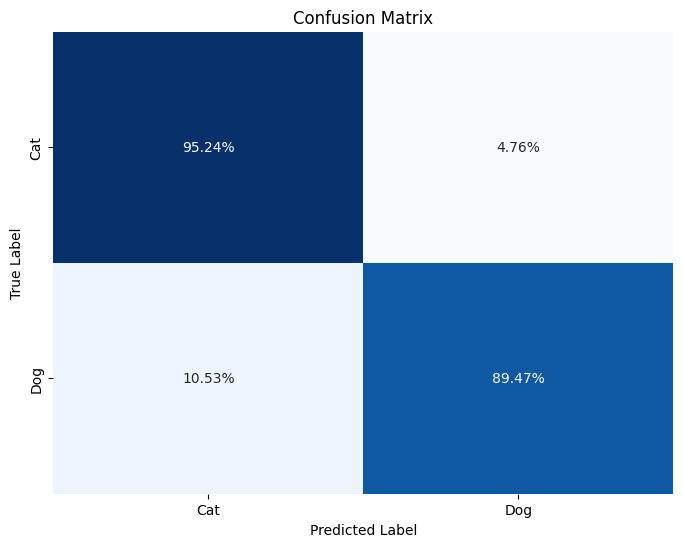
\includegraphics[width=0.5\linewidth]{Figs/conf.png}
    \caption{Matriz de confusión}
    \label{fig:conf}
\end{figure}

Esto indica que el modelo clasificó correctamente 20 maullidos y 17 ladridos, con solo 3 errores en total. Se observa que la mayor parte de los errores provienen de la clasificación errónea de maullidos como ladridos y viceversa, lo que sugiere cierta similitud en algunos patrones espectrales de ambos sonidos.

El rendimiento del modelo también fue evaluado a través de la pérdida en la función de entropía cruzada y la precisión en el conjunto de validación. Durante el entrenamiento, la pérdida disminuyó de manera constante mientras que la precisión aumentó, lo que indica que el modelo fue capaz de aprender patrones relevantes en los datos.

\section{Conclusión}
Se demostró la viabilidad del uso de MFCC y redes neuronales convolucionales para la clasificación de sonidos de animales domésticos. La obtención de una precisión del 93\% indica que la arquitectura utilizada es efectiva para la diferenciación de maullidos y ladridos. Sin embargo, algunos errores en la clasificación sugieren la posibilidad de mejorar el modelo mediante el uso de un conjunto de datos más amplio y variado, lo que permitiría una mejor generalización.

Para futuras investigaciones, se podrían explorar técnicas avanzadas como el uso de modelos de aprendizaje profundo preentrenados, la incorporación de transformadas wavelet para enriquecer las características extraídas o la implementación de estrategias de data augmentation que permitan aumentar la diversidad de los datos de entrenamiento.
% Can use something like this to put references on a page
% by themselves when using endfloat and the captionsoff option.
\ifCLASSOPTIONcaptionsoff
  \newpage
\fi



% trigger a \newpage just before the given reference
% number - used to balance the columns on the last page
% adjust value as needed - may need to be readjusted if
% the document is modified later
%\IEEEtriggeratref{8}
% The "triggered" command can be changed if desired:
%\IEEEtriggercmd{\enlargethispage{-5in}}

% references section

% can use a bibliography generated by BibTeX as a .bbl file
% BibTeX documentation can be easily obtained at:
% http://mirror.ctan.org/biblio/bibtex/contrib/doc/
% The IEEEtran BibTeX style support page is at:
% http://www.michaelshell.org/tex/ieeetran/bibtex/
%\bibliographystyle{IEEEtran}
% argument is your BibTeX string definitions and bibliography database(s)
%\bibliography{IEEEabrv,../bib/paper}
%
% <OR> manually copy in the resultant .bbl file
% set second argument of \begin to the number of references
% (used to reserve space for the reference number labels box)

%\bibliographystyle{IEEEtran} % Estilo de citas de IEEE
%\bibliography{referencias} % Nombre de tu archivo .bib


\end{document}


